\usetikzlibrary{positioning,arrows.meta,quotes,calc}
\tikzset{%
  arrow/.style    = { ->, >=Latex,  line width = 0.4mm, rounded corners, draw = black, every edge/.style={arrow} },
  arrow/.style    = { ->, >=Latex,  very thick, rounded corners, draw = black,
    fill = #1, draw = #1, font = \footnotesize },
  tbox/.style     = { fill = #1!20!white, draw = #1!80!white, thick, align = center,
    minimum width = 1cm, node distance = 1.5cm }
}
\newcommand{\connectall}[2]{
  \foreach \s in {#1} {
    \foreach \t in {#2} {
      \draw[arrow,<->] (\s) -- (\t);
    }
  }
}

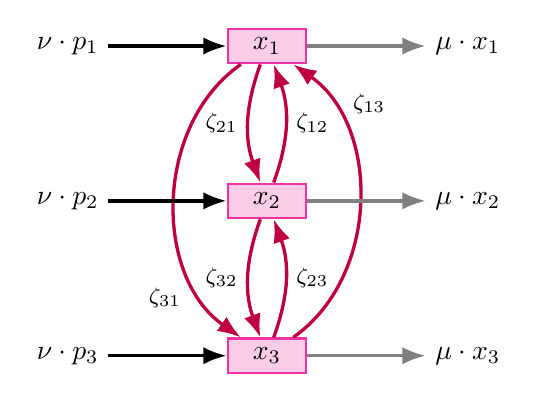
\begin{tikzpicture}
\node(i1) [tbox=magenta] at (0.0,0.0)    {$x_1$};
\node(i2) [tbox=magenta, below = of i1]  {$x_2$};
\node(i3) [tbox=magenta, below = of i2]  {$x_3$};
\node(b1) [left  = 1.5cm of i1] {$\nu \cdot p_1$};
\node(b2) [left  = 1.5cm of i2] {$\nu \cdot p_2$};
\node(b3) [left  = 1.5cm of i3] {$\nu \cdot p_3$};
\node(d1) [right = 1.5cm of i1] {$\mu \cdot x_1$};
\node(d2) [right = 1.5cm of i2] {$\mu \cdot x_2$};
\node(d3) [right = 1.5cm of i3] {$\mu \cdot x_3$};

\draw[arrow=purple] (i1) edge["$\zeta_{21}$", swap, bend right=20] (i2); 
\draw[arrow=purple] (i2) edge["$\zeta_{12}$", swap, bend right=20] (i1);
\draw[arrow=purple] (i3) edge["$\zeta_{23}$", swap, bend right=20] (i2); 
\draw[arrow=purple] (i2) edge["$\zeta_{32}$", swap, bend right=20] (i3);
\draw[arrow=purple] (i1) edge["$\zeta_{31}$", swap, bend right=55, near end] (i3); 
\draw[arrow=purple] (i3) edge["$\zeta_{13}$", swap, bend right=55, near end] (i1);
\draw[arrow=black]  (b1) -- (i1);
\draw[arrow=black]  (b2) -- (i2);
\draw[arrow=black]  (b3) -- (i3);
\draw[arrow=gray]   (i1) -- (d1);
\draw[arrow=gray]   (i2) -- (d2);
\draw[arrow=gray]   (i3) -- (d3);
\end{tikzpicture}